\usepackage{color}\chapter{Implementation}
\label{ch:impl}
\chaptermark{Fourth Chapter Heading}

\definecolor{codegreen}{rgb}{0,0.6,0}
\definecolor{codegray}{rgb}{0.5,0.5,0.5}
\definecolor{codepurple}{rgb}{0.58,0,0.82}
\definecolor{backcolour}{rgb}{0.95,0.95,0.92}
\definecolor{light-gray}{gray}{0.95}

\newcommand{\code}[1]{\colorbox{light-gray}{\texttt{#1}}}
\lstdefinestyle {CodeStyle} {
    basicstyle=\fontfamily{pcr}\small,
    columns=fullflexible,
    showstringspaces=false,
    numbers=left,
    numberstyle=\color{gray}\small,
    stepnumber=1,
    numbersep=10pt,
    backgroundcolor=\color{white},
    showspaces=false,
    showstringspaces=false,
    showtabs=false,
    frame=single,
    xleftmargin=.05\textwidth,
    xrightmargin=.05\textwidth,
    aboveskip=1.5em,
    rulecolor=\color{black},
    tabsize=2,
% captionpos=b,
    breaklines=true,
    breakatwhitespace=false,
% title=\lstname,
    commentstyle=\color{gray}\upshape
}

\lstset{style=CodeStyle}


The following chapter provides details on the implementation of the system, including any issues that arose during the development process and the solutions implemented to address these issues.
Fig.~\ref{fig:architecture} shows the architecture of the implementation of the system.

\begin{figure}[t]
    \centering
    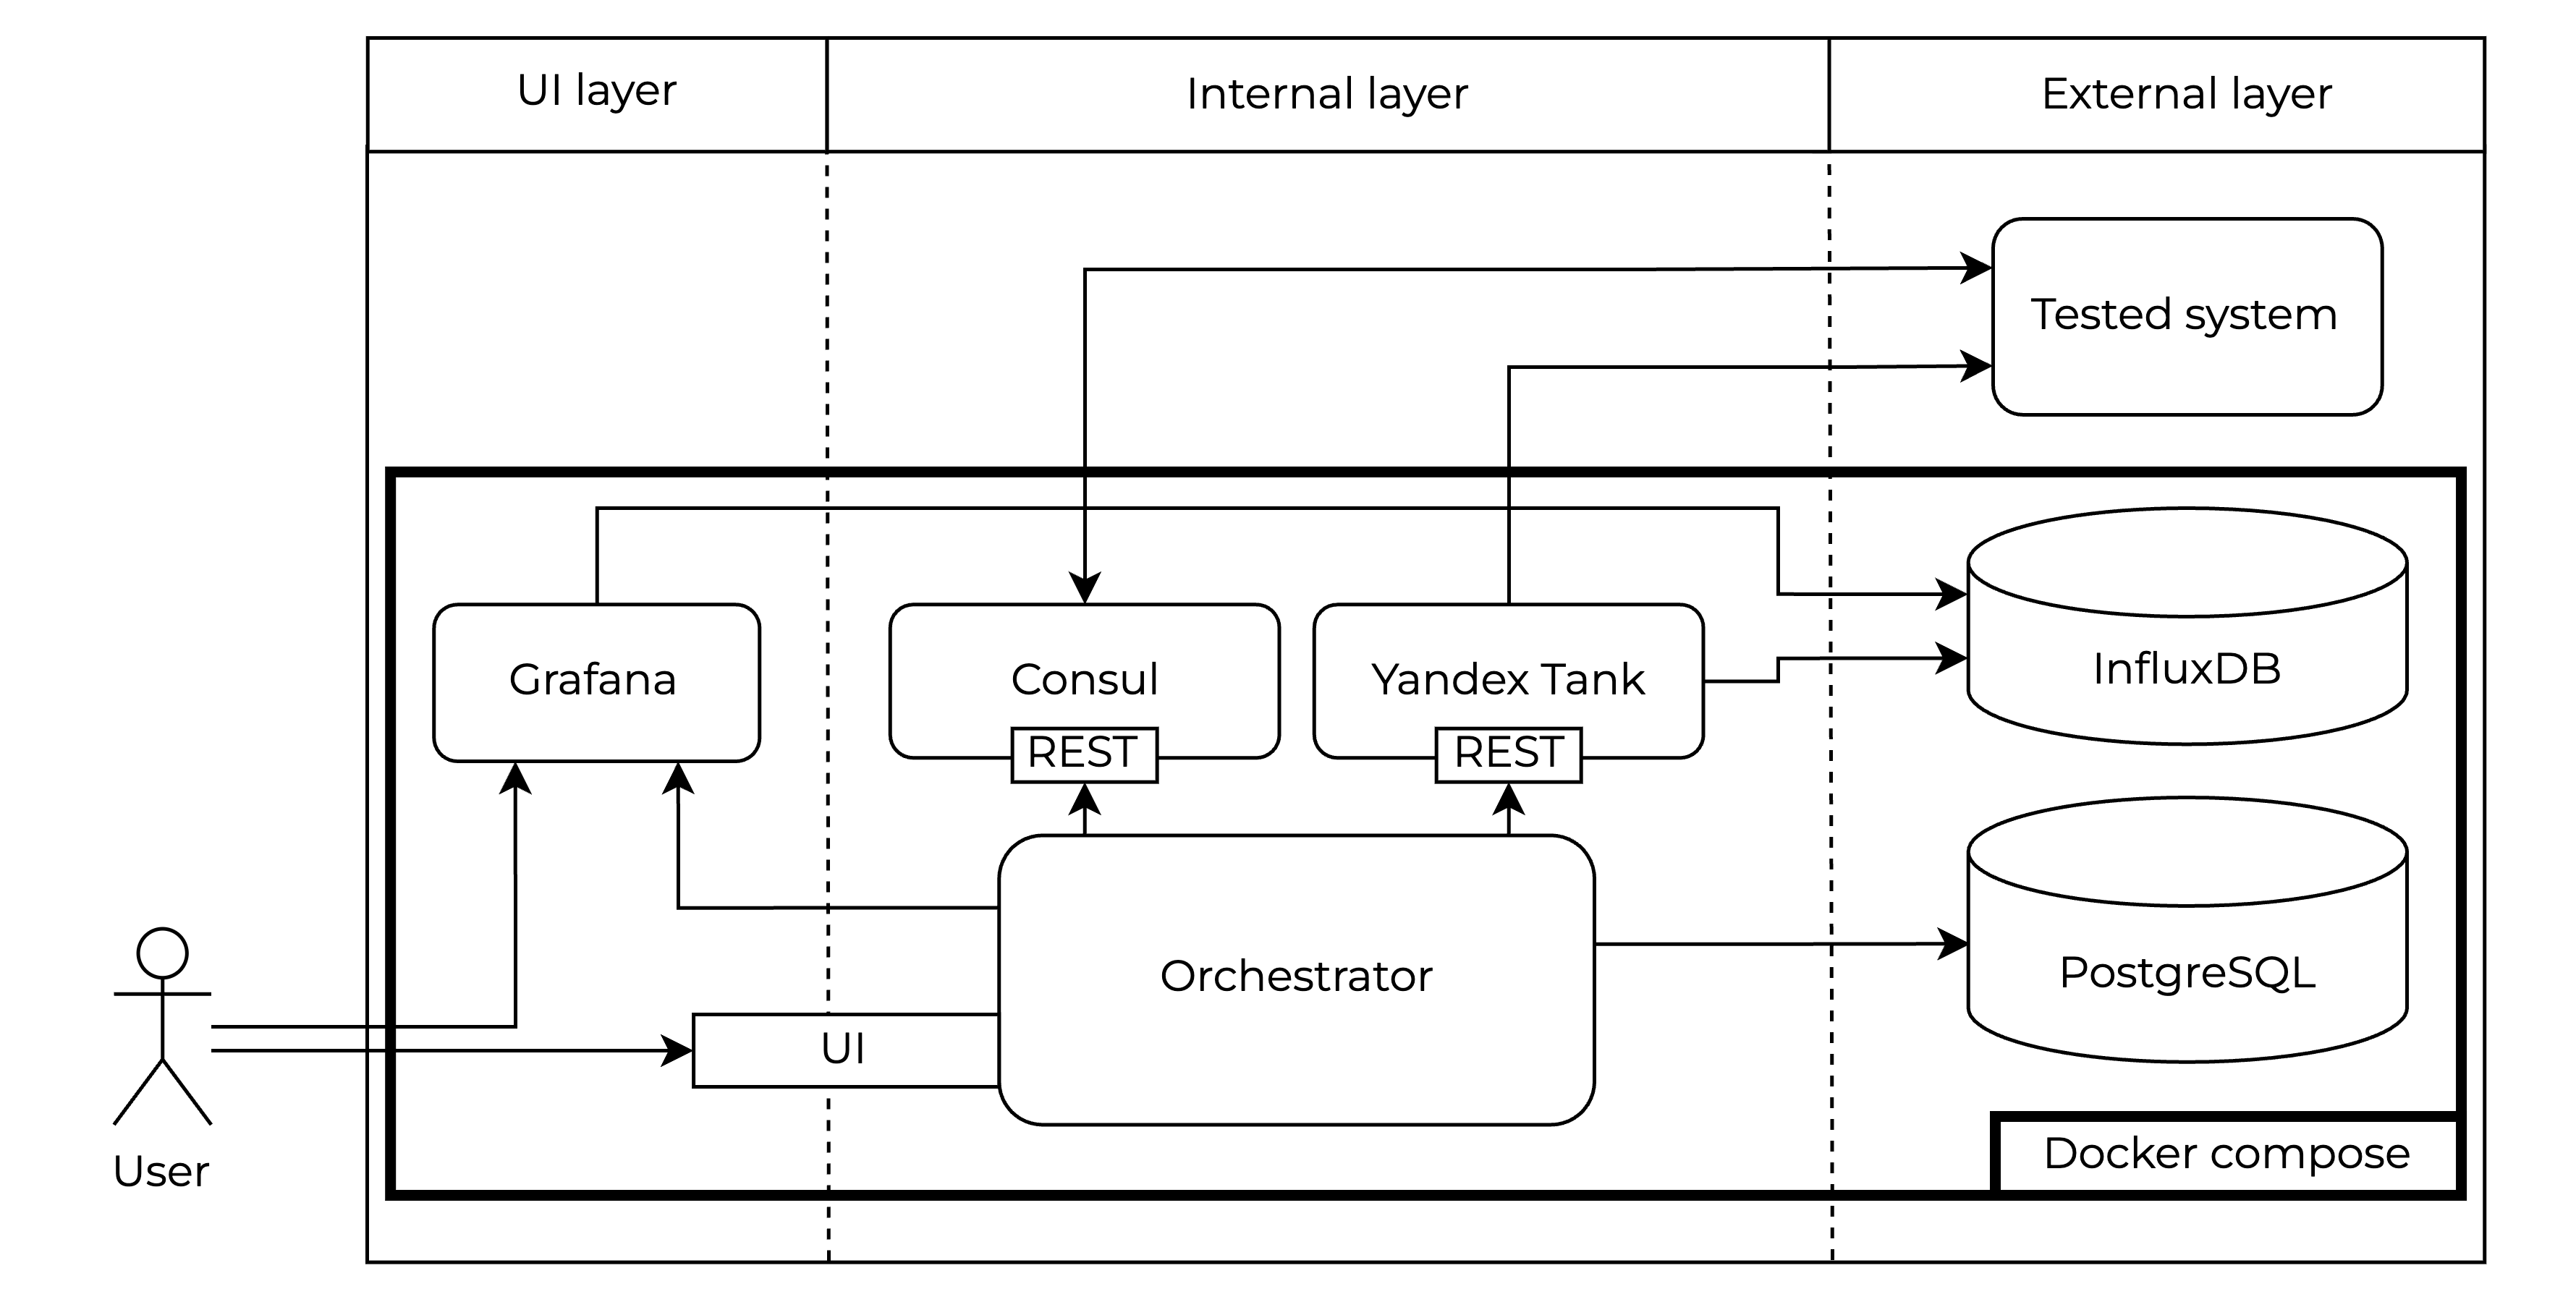
\includegraphics[height=\textheight,width=\textwidth,keepaspectratio]{architecture_v3.png}
    \caption{Architecture of the system}
    \label{fig:architecture}
\end{figure}

\section{Implementation of Load generation module}\label{sec:yandex_tank_use}
Yandex Tank~\cite{yandex_tank} is used as the primary load generation tool in my system. It supports various load generation engines, however, I have chosen Phantom~\cite{phantom} as the defualt engine. Phantom exclusively supports HTTP~\cite{http} requests and may be configured in two distinct ways:
\begin{enumerate}
    \item Single configuration file. This type of configuration only supports HTTP GET~\cite{http} requests.
    \item Configuration file and ammo file. For more complex scenarios with all types of HTTP methods, Phantom~\cite{phantom} supports ammo files. Ammo file contains a sequence of HTTP requests.
\end{enumerate}
Yandex Tank has built-in integration with InfluxDB~\cite{influxdb} and is able to directly write all test results to it.
Yandex Tank API~\cite{yandex_tank_api} is a web server that incapsulates work with Yandex Tank using HTTP API~\cite{microservices}. It is used as an implementation of the load generation module.


\section{Implementation of configuration manager module}
Consul~\cite{consul} is an open-source solution for automating service configuration and discovery. It is used as a configuration manager due to its key/value storage feature. It provides an API for managing key/value storage, and most importantly, Watches~\cite{consul_watches}, which allows all services that are integrated with Consul to receive notifications of any changes to the configuration. It allows to track the impact of configuration changes during load testing.


\section{Implementation of datastore module}\label{sec:implementation-of-datastore}
Datastore is implemented by two database management systems: PostgreSQL~\cite{postgresql} and InfluxDB~\cite{influxdb}.

\subsection{PostgreSQL}\label{subsec:postgresql}
PostgreSQL~\cite{postgresql} is a powerful, open-source object-relational database management system. It is used as the main storage for testing scenarios and metadata about their executions. Fig.~\ref{fig:erd} shows the entity-relationship diagram of the database schema.
\begin{figure}[t]
    \centering
    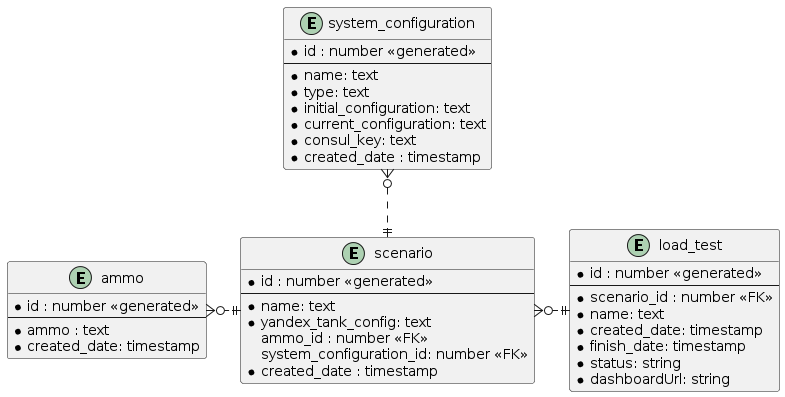
\includegraphics[height=\textheight,width=\textwidth,keepaspectratio]{erd.png}
    \caption{Entity-Relationship Diagram}
    \label{fig:erd}
\end{figure}

Scenarios are stored in three tables:
\begin{enumerate}
    \item \code{scenario} table stores the main information about scenario
    \item \code{system\_configuration} table contains the configuration of the tested system and the key to the Consul key/value storage used to manage the configurations. The initial configuration is the configuration that the system needs at the start of a test, while the current configuration refers to configuration in real time.
    \item \code{ammo} table stores ammo configurations. Ammo is a special term used in Yandex Tank~\cite{yandex_tank}, which is explained in Subsection~\ref{sec:yandex_tank_use}
\end{enumerate}
System configurations and ammo are allocated separately from the main scenario table, as we have a one-to-many relationship (several scenarios may have the same configuration and ammo), and such a relationship should be represented in the form of separate tables to avoid unnecessary data repetitions~\cite{normal_forms}.

Table \code{load\_test} stores metadata about the executions with the following attributes:
\begin{enumerate}
    \item Unique identifier. It is used as main identifier of the execution for storing the result in InfluxDB
    \item Scenario ID. It is a foreign key that references the identifier of the scenario table.
    \item Name of the specific execution.
    \item Created and finish date of the execution.
    \item Status of the execution. Status can be: created, locked, running,  stopped,  failed, finished, starting.
    \item Dashboard URL. The URL is to the Grafana dashboard that visualizes the results of the test.
\end{enumerate}

\subsection{InfluxDB}\label{subsec:influxdb}
InfluxDB~\cite{influxdb} is an open-source time series database management system.
It is used as the main storage for the results of tests due to its integration with Yandex Tank~\cite{yandex_tank}. The results are stored as following time series:
\begin{enumerate}
    \item Response time. It is aggregated with the following quantiles: 100, 99, 95, 90, 75, and 50
    \item Number of threads needed to support a set RPS
    \item Number of responses aggregated with HTTP and Net codes. Net codes are standard codes from POSIX~\cite{posix_errors} used to signal problems with the network.
\end{enumerate}
Additionally, each time series is assigned a unique label that corresponds to the URL of the method used to store the data. For example, if a test involves two HTTP methods, the time series will contain two separate values for each method.
An example of visualizing time series data with different labels is shown in Fig.~\ref{fig:grafana}.


\section{Implementation of Orchestrator module}\label{sec:ochestrator_impl}
Orhestrator module was implemented using Orchestrator service. The development was done using Kotlin~\cite{kotlin} programming language and Spring framework~\cite{spring} for web development.
Hibernate~\cite{hibernate}, a Java library for object-relational mapping, has been utilized to facilitate communication with the PostgreSQL database.
Additionally, Orchestrator service was integrated with Yandex Tank API~\ref{subsec:yandex_tank_api_integration} and Consul~\ref{subsec:consul_integration} service.

\subsection{API}\label{subsec:rest_api}
Orchestrator service provides an HTTP API for creating and managing ammo files, system configurations, scenarios, and load tests.
Table~\ref{tab:rest_api_scenario} provides an example of API for scenarios.
\begin{longtable}[c]{|p{3cm}|p{5cm}|p{7cm}|}
    \caption{API for managing scenarios}
    \label{tab:rest_api_scenario} \\
    \hline    \textbf{HTTP Method} & \textbf{URL} & \textbf{Description} \\
    \endhead    \hline    POST & /api/scenario & Method for creating a scenario. Accept YAML~\cite{yaml} config in the body \\
    \hline    DELETE & /api/scenario & Delete a scenario. All tests with this scenario will be stopped and deleted \\
    \hline    GET & /api/scenario/<id> & Get the scenario by its id
    \hline    GET & /api & Get all scenarios
    \hline
\end{longtable}

\subsection{Integration with Yandex Tank API}\label{subsec:yandex_tank_api_integration}
First of all, Orchestrator service needed to be able to use load testing tool.
I implemented an integration with Yandex Tank API using its HTTP API.
Yandex Tank API stores only information about status of the test, and all other information is stored in PostgreSQL table \code{load\_test}.
Fig.~\ref{fig:creation} illustrates the example of flow for starting the test.
For each test, the Yandex Tank API initializes an instance of Yandex Tank and manages its lifecycle.
The orchestrator periodically polls the status of this lifecycle, as described in the ~\ref{subsec:polling_mechanism}

\begin{figure}[t]
    \centering
    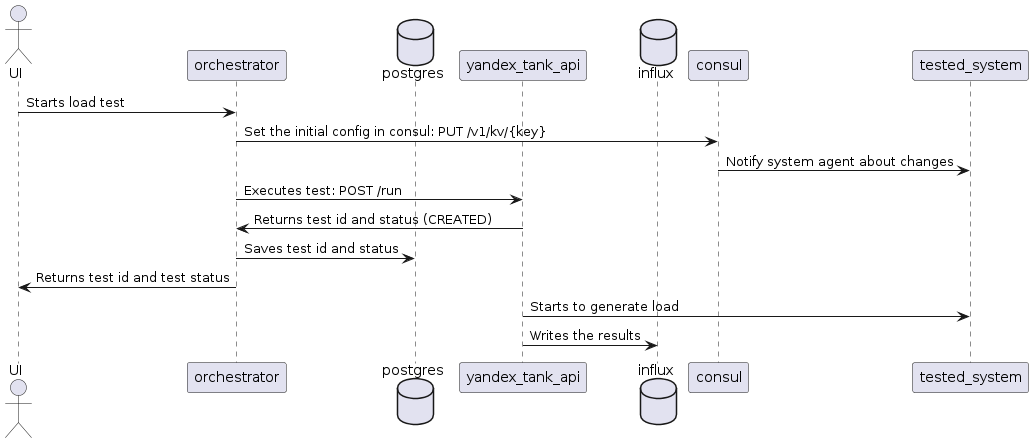
\includegraphics[height=\textheight,width=\textwidth,keepaspectratio]{creation.png}
    \caption{Example of starting the test}
    \label{fig:creation}
\end{figure}

\subsection{Integration with Consul}\label{subsec:consul_integration}
Consul key/value storage provides an HTTP API for managing the configurations. I used this API to read and update configurations in Consul.
At the start of the orchestrator service it establishes a connection with Consul and monitors for any configuration changes using the Watches~\cite{consul_watches} mechanism.

\subsection{Polling mechanism}\label{subsec:polling_mechanism}
To have an actualized status of the load test and configuration of the system, I used HTTP short polling strategy~\cite{http}.
Fig.~\ref{fig:polling} illustrates the process. Every three seconds, the service polls the status and system configuration of unfinished tests and updates them accordingly.
For this purpose, I used a Spring mechanisms for scheduling tasks. The code of the polling mechanism is presented in Listing~\ref{lst:polling}.
\begin{figure}[t]
    \centering
    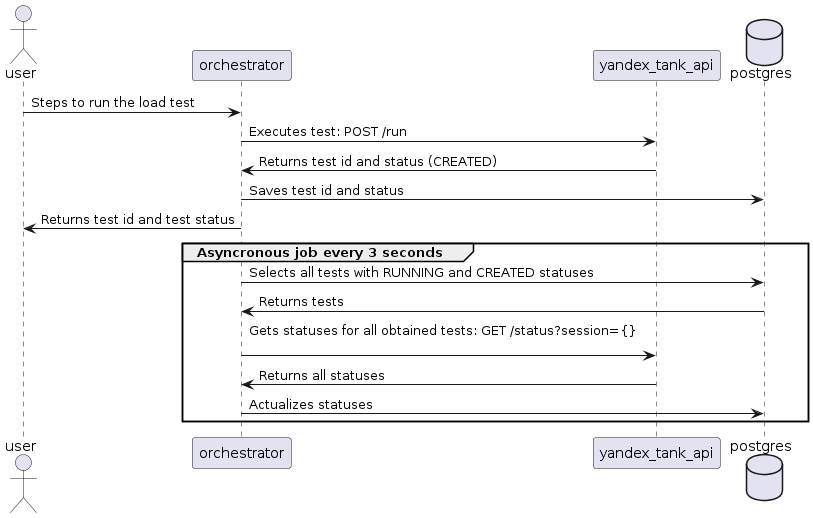
\includegraphics[height=\textheight,width=\textwidth,keepaspectratio]{polling.png}
    \caption{Polling mechanism}
    \label{fig:polling}
\end{figure}

\begin{flushright}
\begin{minipage}{\textwidth}
    \lstinputlisting[language=Kotlin, caption=Polling function, label={lst:polling}]{code/polling.kt}
\end{minipage}
\end{flushright}


\section{Implementation of UI}\label{sec:implementation-of-ui}
UI module is implemented using Grafana~\cite{grafana} and Vaadin~\cite{vaadin} services.
Subsection~\ref{subsec:visualization-of-the-results} presents solution for the visualization of the results using Grafana.
Subsection~\ref{subsec:ui-of-the-orchestrator} describes the implementation of the user interface for the orchestrator.

\subsection{Visualization of the results}\label{subsec:visualization-of-the-results}
One of the most popular way of visualizing the results of the Yandex Tank executions is Overload service~\cite{overload}. It is the distinct web service that store and visualize the results. The problem with using it is the immutability of the chart.
For example, it is not currently possible to create a new chart with a specific aggregation of metrics that would be useful for a particular test. Furthermore, all results are stored within data stores of the Overload and the responsibility for management of this data lies with this service.
As my system stores all test results in InfluxDB, users of my service have full access to it and are able to visualize and aggregate it as they see fit.
I used the Grafana tool~\cite{grafana} for visualization and implemented a custom dashboard with charts that can be easily modified through the UI of the Grafana. Fig.~\ref{fig:grafana} demonstrates an example of the results on my dashboard.

\begin{figure}[t]
    \centering
    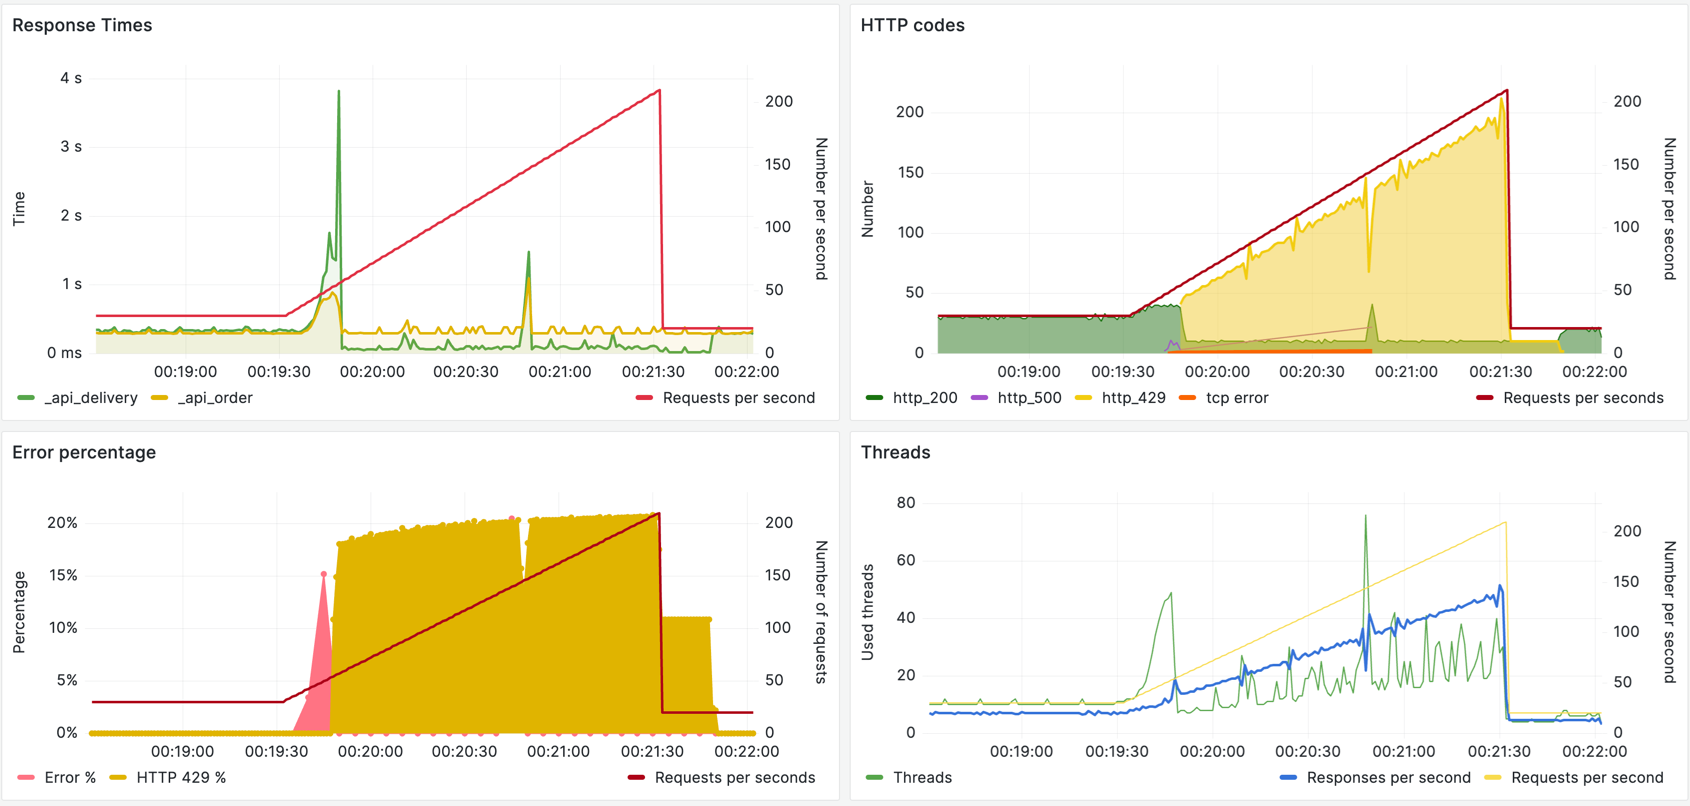
\includegraphics[height=\textheight,width=\textwidth,keepaspectratio]{grafana_v2.png}
    \caption{Example of the charts in Grafana}
    \label{fig:grafana}
\end{figure}

\subsection{UI of the orchestrator}\label{subsec:ui-of-the-orchestrator}
Orchestrator needs a user interface for more convenient use of the service. Vaadin~\cite{vaadin} is a web application platform that allows developers to create an UI using Kotlin. It incapsulates all front-end development in Kotlin objects. For Orchestrator I developed four views: load tests, scenarios, ammo, and system configurations. Each view contains a table with the data, search field, and a creation form. Fig.~\ref{fig:ui} demonstrates example of the load test view.

\begin{figure}[t]
    \centering
    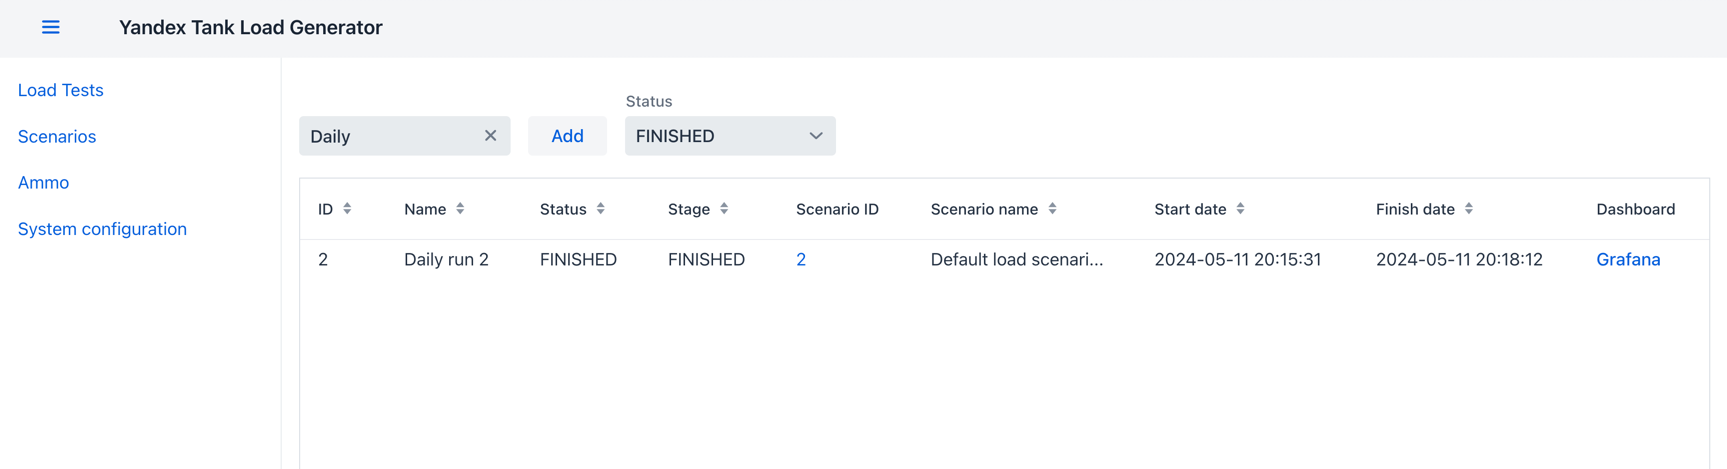
\includegraphics[height=\textheight,width=\textwidth,keepaspectratio]{ui.png}
    \caption{Example of the UI of the orchestrator}
    \label{fig:ui}
\end{figure}
%\begin{figure}[t]
%    \centering
%    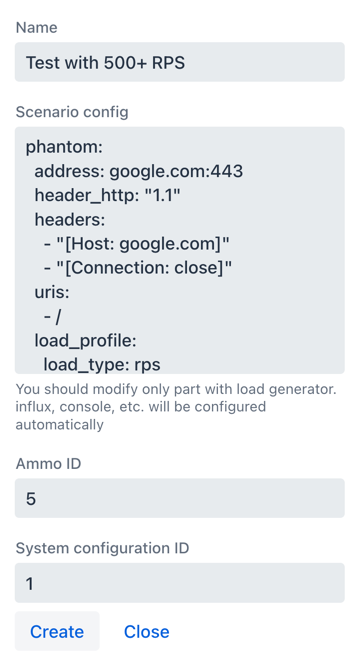
\includegraphics[height=\textheight,width=\textwidth,keepaspectratio]{creation_form.png}
%    \caption{Form for creation scenarios}
%    \label{fig:form}
%\end{figure}

\subsection{Infrastructure}\label{subsec:infrastructure}
Docker~\cite{docker_start} image is a lightweight, standalone, and executable package that contains everything needed to run an application, including the code, runtime, libraries, and system tools. Docker container is an instance of a Docker image that is running in isolation on a host operating system.
For easier deployment and management of the described services, each service has been packaged into a Docker image. Grafana, Consul, InfluxDB and PostgreSQL services already have built images, but Yandex Tank API and Orchestrator needed to be built. For the Yandex Tank API image I used the default image of Yandex Tank~\cite{yandex_tank_image} as based image, then tuned the system parameters for better performance, installed all dependencies, and ran the Yandex Tank API server. For Orchestrator, I first built a JAR file for my project using Gradle~\cite{gradle}, and then using a base image with the Java Runtime Environment installed, execute the compiled JAR file.

Container orchestrating is the automated management of containerized applications, handling deployment, scaling, and operation across multiple hosts. It ensures efficient resource usage, high availability, and scalability.
Docker compose~\cite{docker_compose} is container orchestrating tool for Docker containers, which allows to describe all deployment as a single YAML~\cite{yaml} file. Listing~\ref{lst:docker_compose} illustrates a part of this file for Orchestrator and PostgreSQL containers.
\lstinputlisting[caption=Part of the Docker Compose file, label={lst:docker_compose}]{code/docker-compose.yaml}


\section{Conclusion}\label{sec:conclusion}
The system is implemented using the Yandex Tank API, Consul, Grafana, PostgreSQL, and InfluxDB tools. The Orchestrator web service was developed using Kotlin and Spring. Additionally, all the services was packed into Docker images, and the infrastructure of the application was up using these images with Docker Compose.
